\section*{L'entreprise et son secteur d'activité}
\paragraph{Sogeti et l'ESEC}
\subparagraph{Sogeti}
\begin{figure}[h]
    \centering
    
\includegraphics[scale=0.7]{images/sogeti.png}
    \caption{Logo Sogeti.}
\end{figure}
Sogeti est une Entreprise de Service du Numérique (ESN), filiale appartenant
à 100\% à Capgemini. Sogeti est initialement l'acronyme pour "Société pour la Gestion de
l'Entreprise et le Traitement de l'Information". Fondée en 1967 à Grenoble par Serge Kampf, elle opère
dans 15 pays avec 25 000 collaborateurs, dont environ 6200 en France. Les partenariats sont néggociés au niveau
du groupe (RSA, IBM, CA Tech, Fortinet, etc..).

\subparagraph{European Security Expertise Center}
\begin{figure}[h]
    \centering
    
\includegraphics[scale=0.4]{images/esec.png}
    \caption{Logo ESEC.}
\end{figure}
L'European Security Expertise Center (ESEC), est le pôle responsable des domaines
liés à la sécurité de Sogeti. Le centre est composé plusieurs équipes, dont un
laboratoire de recherche et développement, ou une équipe dédiée aux tests d'intrusion.
C'est dans cette dernière équipe que le stage s'est déroulé.
L'ESEC est directement placé sous le pôle sécurité de Capgemini, dirigé par Frank
Greverie, secondé par Jean Marc Bianchini pour Sogeti.

\begin{figure}[h]
    \centering
    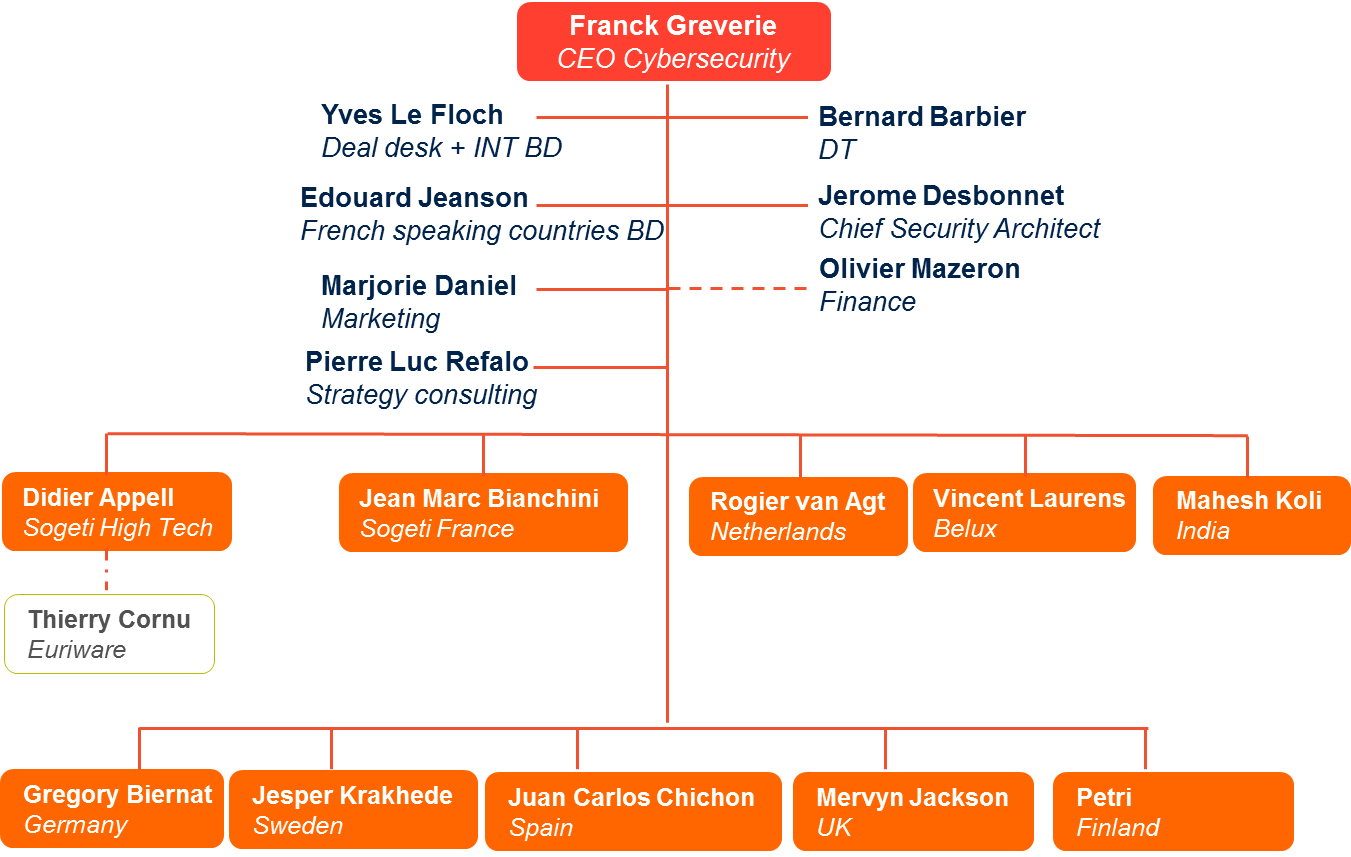
\includegraphics[scale=0.5]{images/organigramme.png}
    \caption{Organisation de la sécurité - Sogeti.}
\end{figure}
\begin{figure}[h]
    \centering
    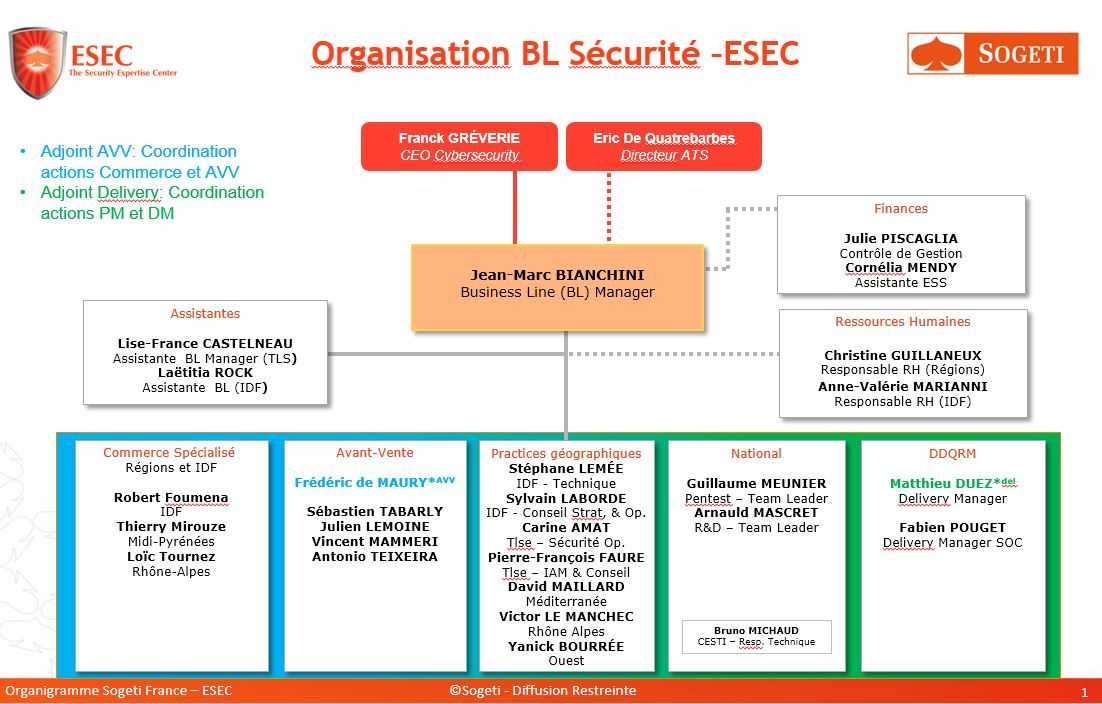
\includegraphics[scale=0.5]{images/bl-esec-orga.png}
    \caption{Organisation Buisiness Line Sécurité - ESEC.}
\end{figure}

\subparagraph{}
Au niveau France, Sogeti et l'ESEC ont plusieurs concurrents, dont Solucom, Deloitte,
et HSC. Le domaine de la sécurité informatique étant en pleine expansion, de nombreuses ESN existante
essayent de développer leurs équipes dans le domaine, afin de gagner des parts de marché
sur des sujets de plus en plus demandeur en terme de force salariale.

\subparagraph{}
Depuis 2014, l'ESEC bénéficie de la certification PASSI (Prestataires d'Audit de la Sécurité
des Systèmes d'Information) délivrée par l'ANSSI (Agence Nationale de la Sécurité des Systèmes
d'Information). Plusieurs autres sociétés ont également cette certification (Bull, CGI, HSC, Solucom, etc.).
Sogeti ESEC est également accréditée pour effectuer des évaluations CSPN.

\begin{figure}[h]
    \centering
    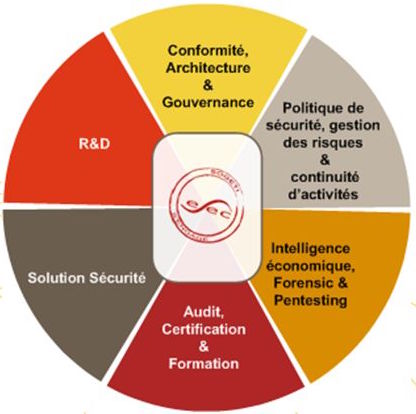
\includegraphics[scale=0.5]{images/activities.jpg}
    \caption{Activités de l'ESEC.}
\end{figure}

\section*{Le service: Tests d'intrusion / Pentest}
Le service dans lequel s'est effectué le stage est celui du test d'intrusion. Il est dirigé par Guillaume Meunier et est composé
de plusieurs bureaux (Toulouse, Paris et Lyon). Sur Paris, l'équipe compte actuellement une dizaine de personnes. Tous les domaines de l'audit de
sécurité sont traités dans cette équipe (audit de code, de configuration, tests d'intrusion interne/externe, etc.).

\subparagraph{}

\section*{État des connaissances avant le stage sur le sujet}
\paragraph{}
Le cursus de la majeure SRS au sein de l'EPITA a pour but d'apporter une base technique et fonctionnelle
sur la sécurité. En corrélation avec le niveau général de la promotion, les points abordés peuvent être
plus ou moins avancés. Le sujet de stage portait sur de l'analyse statique de programme binaire, sans rapports
d'outils externes, pour la détection de vulnérabilité de type "usage-après-libération" (use-after-free).
\subparagraph{}
Les pré-requis sont donc:
\begin{itemize}
\item L'analyse statique instrumentalisée.
\item La compréhension du fonctionnement des allocateurs de mémoire.
\item Le principe de teinte de mémoire/registre pour l'analyse statique.
\item Des notions en théorie des graphes.
\item Des notions en rétro-ingénierie.
\end{itemize}

De ces points, la rétro-ingénierie et la théorie des graphes sont suffisamment enseignées à l'EPITA,
durant l'année de spécialisation ou bien pendant la première année du cycle ingénieur.
\subparagraph{}
Concernant les autres points, l'analyse statique instrumentalisée, en comparaison avec ce qui a été
fait durant le stage, n'était après retour pas très avancée, et les bases étaient difficilement acquises par
l'ensemble de la promotion SRS. Même si le thème de l'analyse statique était bien abordé, le domaine de l'instrumentalisation
aurait peut être eu besoin de plus de temps pour être enseigné et compris. Le principe de teinte mémoire/registre étant intimement
lié à ce dernier point, les commentaires précédents s'y appliquent également.
\subparagraph{}
Le point majoritairement manquant concernant ce stage et la plus grosse lacune concernant le sujet du stage résidait dans la compréhension de
la gestion de la mémoire par un système d'exploitation, des différents niveaux d'allocation mémoire, et de leur fonctionnement précis
selon les cas (niveau noyau ou niveau utilisateur, différents appels, granularité, algorithme de défragmentation/optimisation, ...).
\subparagraph{}
Cette notion est vraiment très peu enseignée durant le cursus de l'EPITA, quelle que soit la spécialisation, même si une partie du projet KSTOS
demandait (à un niveau relativement peu avancé) la compréhension de la relation mémoire physique / mémoire virtuelle.
Les notions et l'étude des ABI (Interface Application-Binaire / Application Binary Interface) est elle aussi assez peu évoquée.
\subparagraph{}

Néanmoins, le premier mois de stage a été dédié à combler ces lacunes et le reste du stage a pu se dérouler avec assez de connaissance
pour être confortable dans ces domaines là.

\subparagraph{}


\section*{Positionnement du stage dans l'entreprise}
\paragraph{}
\subparagraph{}
L'équipe en charge des tests d'intrusion cherche à atteindre plusieurs objectifs à travers leurs offres de stage.
\subparagraph{}
Le stagiaire doit tout d'abord monter en compétence sur un domaine précis afin d'atteindre un niveau au plus proche de l'expertise sur son sujet de stage.\newline
Tout au long du stage se déroulent des présentations d'avancement et/ou de sujets précis dans le cadre du stage, de la part des stagiaires ayant avancé dans leur domaine
et/ou trouver un thème à discuter au sein de l'équipe. Ceci fait partie d'une des attentes de l'équipe envers ses stagiaires: la diffusion de la connaissance acquise.
\subparagraph{}
En complément de ces deux objectifs vient naturellement l'envie de dévelop-per des solutions internes pouvant être réutilisées/améliorées après le stage. Selon la difficulté du sujet de stage
et/ou des compétences du stagiaire, la solution finale sera soit directement utilisée par l'équipe ou reprise par quelqu'un après le stage.\newline

Concernant le sujet du stage présenté dans ce rapport, le type de vulnérabilité, bien que connu de la majorité de l'équipe, restait assez complexe à comprendre en détail,
notamment de part les connaissances en système et conception d'allocateurs mémoire requises. Avoir un stagiaire dans ce domaine permettait donc d'avoir des
rappels / formations sur ces points-là lors des différentes présentations.
